% =====================================================================
\chapter{Copules}
\label{ch:9}
% =====================================================================

\section{Objectifs et organisation du chapitre}

\paragraph{Objectifs.} La corrélation résume la dépendance entre deux actifs par un seul nombre, qui ne dit rien des extrêmes : deux actions peuvent être modérément corrélées en temps normal et chuter ensemble lors des krachs. Les copules séparent la loi de chaque actif (sa \og marge\fg) de la structure de dépendance. À la fin du chapitre, vous saurez : (1) énoncer le théorème de Sklar ; (2) mesurer la dépendance par le tau de Kendall et la dépendance de queue ; (3) manipuler les copules gaussienne, de Student et de Clayton ; (4) estimer une copule et choisir entre plusieurs ; (5) construire les signaux de trading proposés par \citet{liewwu2013} et \citet{xie2016} et juger honnêtement de leur intérêt.

\paragraph{Code.} \texttt{code/ch09/ch09\_copulas.py}, expériences E1 à E4.

% =====================================================================
\section{Définition et théorème de Sklar}
% =====================================================================

\subsection{Copule}

\begin{definition}
Une \emph{copule} bivariée est une fonction de répartition $C : [0,1]^2\to[0,1]$ d'un couple $(U,V)$ dont les deux marges sont uniformes sur $[0,1]$ : $C(u,v) = \Prob(U\le u, V\le v)$, avec $C(u,1) = u$ et $C(1,v) = v$.
\end{definition}

\subsection{La transformation par la fonction de répartition}

Si $X$ a une fonction de répartition continue $F_X$, alors $U = F_X(X)$ est uniforme sur $[0,1]$. En effet, $\Prob(U\le u) = \Prob(F_X(X)\le u) = \Prob(X\le F_X^{-1}(u)) = F_X(F_X^{-1}(u)) = u$. Cette transformation enlève à $X$ tout ce qui tient à sa loi propre (volatilité, épaisseur des queues) et ne garde que son \emph{rang}.

\begin{theorem}[Sklar]\label{c9:thm:sklar}
Pour tout couple $(X,Y)$ de fonction de répartition jointe $H$ et de marges continues $F_X$, $F_Y$, il existe une unique copule $C$ telle que
\[
H(x,y) = C\big(F_X(x), F_Y(y)\big).
\]
Réciproquement, toute copule combinée à deux marges quelconques définit une loi jointe valide.
\end{theorem}
\begin{proof}[Idée de la démonstration]
On pose $U = F_X(X)$ et $V = F_Y(Y)$, uniformes d'après ce qui précède, et $C$ la loi jointe de $(U,V)$. Alors $H(x,y) = \Prob(X\le x, Y\le y) = \Prob(U\le F_X(x), V\le F_Y(y)) = C(F_X(x),F_Y(y))$, car $F_X$ et $F_Y$ sont croissantes.
\end{proof}

\begin{intuition}
Une loi jointe, c'est une recette avec deux ingrédients séparables : la \og forme\fg{} de chaque actif (ses marges) et la \og façon dont ils dansent ensemble\fg{} (la copule). On peut garder les mêmes danseurs et changer de chorégraphie, ou l'inverse.
\end{intuition}

\subsection{Mesures de dépendance}

\paragraph{Tau de Kendall.} Pour deux observations indépendantes $(X_1,Y_1)$ et $(X_2,Y_2)$ du couple, $\tau = \Prob\big((X_1-X_2)(Y_1-Y_2)>0\big) - \Prob\big((X_1-X_2)(Y_1-Y_2)<0\big)$ : la probabilité que deux observations soient rangées dans le même ordre sur les deux actifs, moins celle qu'elles soient en ordre inverse. Il ne dépend que de la copule (les rangs ne changent pas si l'on applique une fonction croissante aux marges).

\paragraph{Dépendance de queue.} La dépendance de queue inférieure est
\[
\lambda_L = \lim_{q\to0}\Prob\big(V\le q\mid U\le q\big),
\]
la probabilité qu'un actif soit dans ses pires $q\,\%$ sachant que l'autre l'est, quand $q$ devient très petit. On définit de même $\lambda_U$ pour les hausses extrêmes.

\subsection{Trois familles}

\begin{table}[h]
\centering\small
\caption{Trois copules usuelles. $\Phi$ : fonction de répartition normale ; $t_\nu$ : loi de Student à $\nu$ degrés de liberté.}
\label{c9:tab:families}
\begin{tabular}{llll}
\toprule
Copule & Paramètre et lien avec $\tau$ & $\lambda_L$ & $\lambda_U$ \\
\midrule
Gaussienne & $\rho = \sin(\pi\tau/2)$ & 0 & 0 \\
Student ($\nu$) & $\rho = \sin(\pi\tau/2)$ & $2\,t_{\nu+1}\!\Big(-\sqrt{\frac{(\nu+1)(1-\rho)}{1+\rho}}\Big)$ & idem \\
Clayton & $\theta = 2\tau/(1-\tau)$ & $2^{-1/\theta}$ & 0 \\
\bottomrule
\end{tabular}
\end{table}

La copule de Clayton s'écrit $C(u,v) = (u^{-\theta} + v^{-\theta} - 1)^{-1/\theta}$ : elle concentre la dépendance dans les baisses communes. La copule gaussienne n'a aucune dépendance de queue : quels que soient $\rho<1$, les extrêmes deviennent asymptotiquement indépendants.

\begin{codebox}[ — E1, même $\tau$, extrêmes différents]
\textbf{Protocole :} 400\,000 tirages de chaque copule avec $\tau = 0{,}5$. \textbf{Résultats :} probabilité que les deux actifs soient simultanément dans leur pire 1\,\% : $0{,}27\,\%$ (gaussienne), $0{,}45\,\%$ (Student, $\nu = 4$), $0{,}70\,\%$ (Clayton), contre $0{,}01\,\%$ sous indépendance. Probabilité conditionnelle $\Prob(V<1\,\%\mid U<1\,\%)$ : $0{,}27$ ; $0{,}45$ ; $0{,}70$. Pour les hausses extrêmes, Clayton tombe à $0{,}03\,\%$. Dépendances de queue théoriques : 0 ; $0{,}40$ ; $0{,}71$.
\end{codebox}

\begin{figure}[h]
\centering
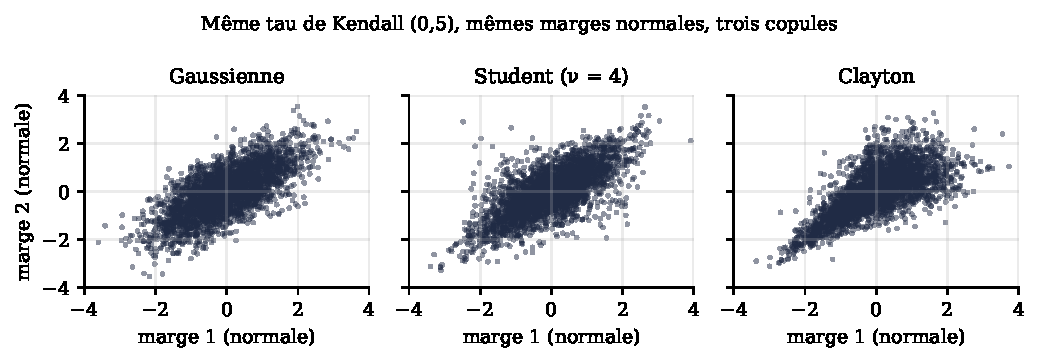
\includegraphics[width=0.98\textwidth]{ch09/trois_copules.pdf}
\caption{Trois copules de même tau de Kendall, représentées avec des marges normales. La Clayton resserre les points dans le coin inférieur gauche (baisses simultanées).}
\label{c9:fig:three}
\end{figure}

\paragraph{Lecture pour le trading.} Une paire couverte avec un ratio estimé en temps normal est exposée à ce qui se passe dans les queues. Si la dépendance de queue est forte, les deux jambes chutent ensemble et la couverture tient ; si elle est faible (une jambe chute seule), l'écart explose. Le choix de la copule est donc d'abord une question de \emph{gestion du risque}.

% =====================================================================
\section{Estimation et choix de la copule}
% =====================================================================

\paragraph{Pseudo-observations.} On ne connaît pas les marges exactes ; on les remplace par les rangs : $\hat u_i = \mathrm{rang}(x_i)/(n+1)$. Diviser par $n+1$ plutôt que $n$ évite les valeurs 0 et 1, où les densités de copule peuvent être infinies.

\paragraph{Paramètre.} Le plus simple est d'inverser la relation entre $\tau$ et le paramètre (tableau~\ref{c9:tab:families}) ; le plus précis est le maximum de vraisemblance sur la densité de copule $c(u,v) = \partial^2C/\partial u\partial v$.

\paragraph{Choix.} On compare les familles par le critère d'Akaike, $\mathrm{AIC} = 2k - 2\ell$, où $k$ est le nombre de paramètres et $\ell$ la log-vraisemblance maximale ; plus petit est meilleur.

\begin{codebox}[ — E2, estimation et choix par AIC]
\textbf{Protocole :} 100 échantillons de 500 observations pour chaque vraie copule ($\tau = 0{,}5$). \textbf{Résultats :} la bonne famille est choisie 98 fois sur 100 (gaussienne), 100 fois (Student), 100 fois (Clayton) ; les paramètres estimés par inversion de $\tau$ valent en moyenne $0{,}710$ (vrai $0{,}707$), $0{,}704$ et $2{,}011$ (vrai $2$).
\end{codebox}

% =====================================================================
\section{Signaux de trading fondés sur les copules}
% =====================================================================

\subsection{La probabilité conditionnelle}

La quantité clé est la \emph{fonction $h$} : $h(u\mid v) = \Prob(U\le u\mid V = v) = \partial C(u,v)/\partial v$. Si $h(u_t\mid v_t)$ est proche de 1, l'actif $X$ a fait \og trop bien\fg{} aujourd'hui compte tenu de ce qu'a fait $Y$ ; proche de 0, trop mal.

\begin{proposition}[Fonction $h$ gaussienne]\label{c9:prop:hgauss}
Pour la copule gaussienne de paramètre $\rho$, $h(u\mid v) = \Phi\Big(\dfrac{\Phi^{-1}(u) - \rho\,\Phi^{-1}(v)}{\sqrt{1-\rho^2}}\Big)$.
\end{proposition}
\begin{proof}
Posons $A = \Phi^{-1}(U)$ et $B = \Phi^{-1}(V)$ : le couple $(A,B)$ est gaussien centré réduit de corrélation $\rho$. D'après le lemme~\ref{c8:lem:cond}, sachant $B = b$, $A$ suit $\N(\rho b, 1-\rho^2)$. Donc $\Prob(U\le u\mid V=v) = \Prob(A\le\Phi^{-1}(u)\mid B = \Phi^{-1}(v)) = \Phi\big((\Phi^{-1}(u)-\rho\Phi^{-1}(v))/\sqrt{1-\rho^2}\big)$.
\end{proof}

Pour Clayton, en dérivant $C$ par rapport à $v$ : $h(u\mid v) = v^{-\theta-1}(u^{-\theta}+v^{-\theta}-1)^{-1/\theta-1}$.

\subsection{Deux règles de la littérature}

\begin{itemize}
\item \citet{liewwu2013} : on calcule chaque jour $h(u_t\mid v_t)$ et $h(v_t\mid u_t)$ sur les rendements ; si la première est inférieure à $0{,}05$ et la seconde supérieure à $0{,}95$, $X$ est jugé sous-évalué par rapport à $Y$ : on achète $X$ et vend $Y$.
\item \citet{xie2016} : on cumule les \og indices de mauvaise évaluation\fg{} $m_t = h(u_t\mid v_t) - 0{,}5$ dans le temps ; on ouvre quand les indices cumulés des deux actifs dépassent un seuil dans des sens opposés et on ferme quand ils reviennent à zéro.
\end{itemize}

\begin{codebox}[ — E3, signal de copule cumulé contre \emph{z-score}]
\textbf{Protocole :} 60 paires simulées, cointégrées en log-prix (écart AR(1), $\varphi = 0{,}9$), chocs de Student à 3 degrés de liberté ; formation de 500 jours (estimation de la copule sur les rendements : la copule de Student est retenue 60 fois sur 60) ; trading de 500 jours ; coûts de 5 pb par jambe. \textbf{Résultats} (gain sur 500 jours, en \% du notionnel brut) : \emph{z-score} sur l'écart $9{,}1\,\%$ (écart-type $4{,}6\,\%$) ; signal de copule cumulé (seuil $0{,}6$) $1{,}6\,\%$ (écart-type $2{,}3\,\%$).
\end{codebox}

\paragraph{Pourquoi la copule fait moins bien ici.} Une copule estimée sur des rendements quotidiens décrit leur dépendance \emph{instantanée}. Si les rendements sont indépendants d'un jour à l'autre, la copule ne contient aucune information sur l'avenir : un \og rendement trop haut\fg{} n'est pas suivi d'une correction. Le signal ne gagne que dans la mesure où l'indice cumulé reconstruit l'écart de niveau, ce que le \emph{z-score} fait directement. \citet{rad2016} trouvent de même que la méthode par copules n'est pas plus rentable que les méthodes par distance et cointégration, même si son profil de risque diffère.

\begin{pitfall}
La copule n'est pas une source de rendement en soi. Elle n'apporte un avantage que si la structure de dépendance contient une information de retour à la moyenne que l'écart linéaire ignore. Son usage le plus robuste est ailleurs : modéliser les co-extrêmes pour dimensionner les positions et placer les stop-loss (chapitre~17).
\end{pitfall}

% =====================================================================
\section{Étude de cas réelle : KO et PEP}
% =====================================================================

\begin{codebox}[ — E4, copule des rendements quotidiens KO/PEP]
Sur 499 rendements quotidiens : $\tau = 0{,}449$. Log-vraisemblances : gaussienne $121{,}4$, Student ($\nu = 4$) $114{,}5$, Clayton $46{,}5$ : l'AIC retient la gaussienne. Jours où les deux titres sont simultanément dans leurs pires 5\,\% : 5 observés, contre 8,6 attendus avec la copule gaussienne ajustée, 10,8 avec la Student, 16,4 avec la Clayton et 1,2 sous indépendance.
\end{codebox}

Sur cette période, les deux titres n'ont pas eu plus de baisses communes extrêmes que ne le prévoit une copule gaussienne. Avec seulement cinq événements, l'incertitude est énorme : un seul épisode de stress aurait pu changer la conclusion. Pour estimer des queues, il faut des historiques longs.

% =====================================================================
\section{Ce que la théorie apporte, et ses limites}
% =====================================================================

\paragraph{Apports.} Séparation propre entre marges et dépendance, mesures de dépendance robustes (rangs), modélisation explicite des co-extrêmes, probabilités conditionnelles interprétables.

\paragraph{Limites.} La copule est statique : elle ne modélise pas la dynamique de retour à la moyenne qui fait gagner un \emph{pairs trade}. Les queues sont estimées sur très peu de points. Le choix de la famille est un a priori fort ; les copules à paramètres variables dans le temps sont plus réalistes mais beaucoup plus difficiles à estimer.

% =====================================================================
\section{Fiche à recopier au tableau blanc}
% =====================================================================

\begin{whiteboard}
\begin{itemize}[leftmargin=1.2em]
\item \textbf{Transformation :} $U = F_X(X)\sim\mathcal U[0,1]$.
\item \textbf{Sklar :} $H(x,y) = C(F_X(x),F_Y(y))$.
\item \textbf{Kendall :} $\tau = \Prob(\text{concordance}) - \Prob(\text{discordance})$ ; gaussienne/Student : $\rho = \sin(\pi\tau/2)$ ; Clayton : $\theta = 2\tau/(1-\tau)$.
\item \textbf{Queue :} $\lambda_L = \lim_{q\to0}\Prob(V\le q\mid U\le q)$ ; Clayton $2^{-1/\theta}$ ; gaussienne 0.
\item \textbf{Clayton :} $C = (u^{-\theta}+v^{-\theta}-1)^{-1/\theta}$.
\item \textbf{Fonction $h$ :} $h(u|v) = \partial C/\partial v$ ; gaussienne $\Phi\big((\Phi^{-1}(u)-\rho\Phi^{-1}(v))/\sqrt{1-\rho^2}\big)$.
\item \textbf{Pseudo-observations :} rang$/(n+1)$ ; choix par AIC $= 2k-2\ell$.
\end{itemize}
\end{whiteboard}

% =====================================================================
\section{Exercices}
% =====================================================================

\begin{exercise}
Montrez que la copule d'indépendance est $C(u,v) = uv$ et que son tau de Kendall est nul.
\end{exercise}

\begin{exercise}
Démontrez la formule $\lambda_L = 2^{-1/\theta}$ pour la copule de Clayton en calculant $C(q,q)/q$ et en faisant tendre $q$ vers 0.
\end{exercise}

\begin{exercise}
Dérivez la fonction $h$ de la copule de Clayton à partir de $C(u,v)$.
\end{exercise}

\begin{exercise}[à coder]
Ajoutez la copule de Clayton \og tournée\fg{} (de survie) $\tilde C(u,v) = u + v - 1 + C(1-u,1-v)$, qui a une dépendance de queue supérieure. Mesurez sur KO/PEP si elle améliore l'AIC.
\end{exercise}

\begin{exercise}[à coder]
Modifiez E3 pour que les rendements simulés aient une composante prévisible (par exemple une réaction partielle de $X$ aux chocs de $Y$ du jour précédent). La copule estimée sur les couples $(r^X_{t+1}, r^Y_t)$ fait-elle alors mieux que le \emph{z-score} ?
\end{exercise}

% =====================================================================
\section{Pour aller plus loin}
% =====================================================================

\begin{toread}
\begin{itemize}[leftmargin=1.2em]
\item \citet{liewwu2013} : la première application des copules au \emph{pairs trading}, avec la règle des probabilités conditionnelles.
\item \citet{xie2016} : l'indice de mauvaise évaluation cumulé.
\item \citet{rad2016} : la comparaison de la méthode par copules avec les méthodes par distance et cointégration sur longue période.
\item \citet{krauss2017survey}, partie consacrée aux \og autres approches\fg{} : synthèse des variantes à base de copules.
\end{itemize}
\end{toread}

\section{Scripts du chapitre}
\noindent\texttt{code/ch09/ch09\_copulas.py} : E1 (figure~\ref{c9:fig:three}), E2, E3, E4.
